% Diese Zeile bitte -nicht- aendern.
\documentclass[course=asp]{aspdoc}
\usepackage[ruled, vlined]{algorithm2e}
\usepackage{amsfonts}
\usepackage{pgfplots}
\usepackage{listings}
\pgfplotsset{width=10cm,compat=1.9}
%%%%%%%%%%%%%%%%%%%%%%%%%%%%%%%%%
%% TODO: Ersetzen Sie in den folgenden Zeilen die entsprechenden -Texte-
%% mit den richtigen Werten.
\newcommand{\theGroup}{117} % Beispiel: 42
\newcommand{\theNumber}{A201} % Beispiel: A123
\author{Manuel Schnaus \and Stefan Gruber \and Leonhard Chen}
\date{Wintersemester 2019/20} % Beispiel: Wintersemester 2019/20
%%%%%%%%%%%%%%%%%%%%%%%%%%%%%%%%%

% Diese Zeile bitte -nicht- aendern.
\title{Gruppe \theGroup{} -- Abgabe zu Aufgabe \theNumber}

\begin{document}
\maketitle

\section{Einleitung}
Eine wichtige Fragestellung der Informatik ist die Findung von Kanten in Bildern. Mit diesen Kanten ist es möglich, Abgrenzungen von Objekten und Bereichen in einem Bild zu erkennen, was Algorithmen zur Kantenfindung in vielen Bereichen der Bildverarbeitung zu einem fundamentalen Werkzeug macht. In unserem Projekt implementieren wir den sog. Sobel-Filter. Der Sobel-Filter hebt Umrisse in einem Bild hervor, indem dessen Faltungsoperationen auf das Bild angewendet werden. Dazu haben wir einen Algorithmus in Pseudocode entwickelt, um die Faltungs-operation auf ein Bild im unkomprimierten BMP-Bildformat anzuwenden. Diesen implementieren wir in C und Assembler, um deren Performanz zu vergleichen. Neben der Laufzeitanalyse besteht unsere Aufgabe darin den Sobel-Filter, gegeben als folgende mathematischen Formeln, zu implementieren.
\begin{center}
$A^{v}=M^{v}\ast E$
\end{center}
Das Originalbild $E$ wird zunächst getrennt vertikal und horizontal gefiltert. Im oberen Beispiel wird das vertikale Ausgabebild $A^{v}$ berechnet. Hier ist $\ast$ der Faltungsoperator und $M^{v}$ bzw. $M^{h}$ die Faltungsmatrix, wobei $v$ die vertikale und $h$ die horizontale Matrix indiziert. Die Faltungsmatrizen haben einen Grad von $2k+1\times 2k+1$ (in unserem Fall $k=1$). Die Faltungsoperation ist definiert durch diese Formel
\begin{center}
$A_{(x,y)}^{v,F}=\displaystyle\sum_{i=-k}^{k}\displaystyle\sum_{j=-k}^{k}M_{(k+i,k+j)}^{v}\cdot E_{(x+i,y+j)}^{F}$
\end{center}
Hier ist $A_{(x,y)}^{v,F}$ das Ausgabebild am Punkt $(x,y)$. Das $v$ indiziert, dass jenes Ausgabebild vertikal berechnet wurde. Das $F$ steht wiederum für den jeweiligen Farbkanal vom Ausgabebild. Ein Pixel $p$ an der Position $(x,y)$ definiert sich über die Farbkomponenten RGB i.e. Rot, Grün, Blau.
\begin{center}
$p_{(x,y)}=(R_{(x,y)},G_{(x,y)},B_{(x,y)})$
\end{center}
\newpage
Daher errechnet sich das Ausgabebild mit der Faltungsmatrix $M$ vom Grad $k=1$ über die direkt umliegenden Pixel für die jeweiligen Farbkanäle. Abschließend kann das Gesamtbild $G_{(x,y)}^{F}$ an Position $(x,y)$ für die jeweiligen Farbkanäle $F$ berechnet werden. Dieses besteht aus der Wurzel der Summe der Quadrate beider Ausgabebilder an der jeweiligen Position.
\begin{center}
$G_{(x,y)}^{F}=\sqrt{(A_{(x,y)}^{v,F})^{2}+(A_{(x,y)}^{h,F})^{2}}$
\end{center}

\section{Lösungsansatz}
\subsection{Kernalgorithmus}
Um eine algorithmische Lösung zu finden, wird zunächst die Formel des Sobel-Filters wie in Algorithm 1 gezeigt auf das gesamte Bild angewandt. Hier werden die Randfälle des Bildes zunächst nicht behandelt. Diese werden gesondert in Kapitel 2.2 betrachtet.\\

% Pseudocode
\begin{algorithm}[H]
\caption{Mathematischer Filter-Algorithmus}
 \KwData{Eingabebild $E \in \mathbb{R}^{\text{b} \times \text{h} \times 3}$, Ausgabebild $G \in \mathbb{R}^{\text{b} \times \text{h} \times 3}$, Breite des Bildes $b \in \mathbb{N}$, Höhe des Bildes $h \in \mathbb{N}$}
 $M^h=\left( \begin{array}{rrr}
 1&0&-1\\
 2&0&-2\\
 1&0&-1\\
 \end{array} \right)$, 
 $M^v=\left( \begin{array}{rrr}
 1&2&1\\
 0&0&0\\
 -1&-2&-1\\
 \end{array} \right)$\\
 $y = 1$\\
 \While{$y < \text{h} - 1$}{
  $x = 1$\\
  \While{$x < \text{b} - 1$}{
   $A_{(x,y)}^{v}=\displaystyle\sum_{i=-1}^{1}\displaystyle\sum_{j=-1}^{1}M_{(1+i,1+j)}^{v}\cdot E_{(x+i,y+j)}$\\
   $A_{(x,y)}^{h}=\displaystyle\sum_{i=-1}^{1}\displaystyle\sum_{j=-1}^{1}M_{(1+i,1+j)}^{h}\cdot E_{(x+i,y+j)}$\\
   $G_{(x,y)}=\sqrt{(A_{(x,y)}^{v})^{2}+(A_{(x,y)}^{h})^{2}}$\\
   $x=x+1$\\
  }
  $y=y+1$\\
 }
\end{algorithm}

\noindent Ein auffälliger Aspekt dieses Algorithmus ist, dass bei der Berechnung von $A_{(x,y)}^v$ und $A_{(x,y)}^h$ drei der neun Elemente der Summe mit null multipliziert werden und somit nicht in das Ergebnis einfließen. Um diese redundanten Rechnungen zu vermeiden, wird die Summe zur Berechnung von $A_{(x,y)}^v$ ersetzt durch die Formel
\begin{center}
$A_{(x,y)}^v=E_{(x-1,y-1)}+2 \cdot E_{(x,y-1)}+E_{(x+1,y-1)}-E_{(x-1,y+1)}-2 \cdot E_{(x,y+1)}-E_{(x+1,y+1)}$
\end{center}
Analog wird die horizontale Formel für $A_{(x,y)}^{h}$ ersetzt durch
\begin{center}
$A_{(x,y)}^h=E_{(x-1,y-1)}-E_{(x+1,y-1)}+2 \cdot E_{(x-1,y)}-2 \cdot E_{(x+1,y)}+E_{(x-1,y+1)}-E_{(x+1,y+1)}$
\end{center}
Zusätzlich zu der Aussparung der Null-Elemente hat diese Form den Vorteil, dass keine Speicherzugriffe mehr auf die Faltungsmatrizen durchgeführt werden müssen, was sich wiederum positiv auf die Laufzeit des Algorithmus auswirkt. In der Implementierung findet sich diese Verbesserung in den zwei C-Implementierungen wieder, wobei die Faltungsmatrix bei einer Ausführung mit dem Parameter \texttt{-c} verwendet wird und eine Ausführung mit dem Parameter \texttt{-i} die verbesserte Formel benutzt. In den Implementierungen in Assembler wird hier in jedem Fall die verbesserte Formel angewendet.\\\\
Zudem wird hier sichtbar, dass von den sechs Werten, die für die vertikale Berechnung eines Farbkanals verwendet werden, vier Werte auch für die horizontale Berechnung eines Farbkanals benutzt werden können. Durch diese Zusammensetzung werden für jeden Farbkanal jedes Pixels vier Load-Operationen eingespart, was besonders in der Assembler-Implementierung aktiv genutzt werden kann. Diese Optimierung wird sowohl in dem Assembler-Programm mit SIMD, als auch in dem weniger optimierten Assembler-Programm umgesetzt, wobei sie hier in den Algorithmen nicht explizit aufgeführt wird.\\\\
Nachdem in den bisherigen Formeln mit den Vektoren $A_{(x,y)}^h,A_{(x,y)}^v,E_{(x,y)} \in \mathbb{R}^3$ gerechnet wird, stellt sich nun die Frage, wie diese Vektoren aufgespalten und effizient berechnet werden können. Seien im Folgenden $A^v$ die vertikale Komponente und $A^h$ die horizontale Komponente des Ausgabe-Pixels  $G$. Des Weiteren bezeichnet ein Wert $V^F$ mit $F \in \{R, G, B\}$ einen beliebigen Farbkanal eines RGB-Vektors $V \in \mathbb{R}^3$, wobei $V^R$, $V^G$ und $V^B$ der Rot-, Grün-, und Blau-Anteil von $V$ sind. Damit gilt für die Berechnung eines Pixels im Ausgabebild
\begin{center}
$G=\left(
\begin{array}{c}
G^R\\
G^G\\
G^B\\
\end{array}
\right)=\left(
\begin{array}{c}
\sqrt{(A_{(x,y)}^{v, R})^{2}+(A_{(x,y)}^{h, R})^{2}}\\
\sqrt{(A_{(x,y)}^{v, G})^{2}+(A_{(x,y)}^{h, G})^{2}}\\
\sqrt{(A_{(x,y)}^{v, B})^{2}+(A_{(x,y)}^{h, B})^{2}}\\
\end{array}
\right)$
\end{center}
Hier ist anzumerken, dass die Farbkanäle von $G$ direkt von dem Eingabebild abhängen und nicht miteinander verknüpft sind. Daher ist die naheliegende Lösung, in der Schleife statt über die Pixel über alle Farbkanäle zu iterieren. Aufgrund der hier verwendenden Farbtiefe von 24 Bit werden somit die Input-Daten zunächst byte-weise ausgelesen~\cite{bitmapwiki} und mit Hilfe der Formel für $G_{(x,y)}^F$ verarbeitet.\\\\
Im Folgenden werden weitere Optimierungen erläutert, die lediglich in Assembler umgesetzt werden. Zum einen wird die doppelte Schleife durch eine einfachen Schleife über die momentane Adresse des Eingabebildes ersetzt. Dabei wird für das Überspringen der Randpixel eine Variable eingeführt, die über die Breite zählt. Mit dieser Methode wird die Variable $y$ aus Algorithm 1 nicht mehr benötigt und es können vor allem redundante Befehle zur Bestimmung der Adresse vermieden werden. Außerdem zeigt hier für die Berechnung eines Pixels $G_{(x,y)}$ der Pointer des Inputs auf den Pixel $E_{(x-1,y-1)}$. Dies wird jedoch zunächst weniger zur Steigerung der Performanz gewählt, sondern um einheitliche Zugriffe mit positiven, anfangs gesetzten Offsets zu ermöglichen. In Algorithm 2 wird der daraus resultierende Algorithmus beschrieben, aus welchem die Assembler-Implementierungen hervorgehen.\\\\
\begin{algorithm}[H]
\caption{Optimierter Filter-Algorithmus}
 \KwData{Eingabebild E[], Ausgabebild G[], Breite des Bildes b, Höhe des Bildes h}
 $E_{max} = b \cdot h \cdot 3 -b \cdot 6 - 6+ E$\\
 $w=0$\\
 \While{$E<E_{max}$}{
 \If{$w=3 \cdot (b-2)$}{
  $E=E+6$\\
  $G=G+6$\\
  $w=0$\\
  \textbf{continue}\\
 }
  $A^{v,F}=E[0] + 2 \cdot E[3] + E[6]-E[6 \cdot b]-2 \cdot E[6 \cdot b+3]-E[6 \cdot b+6]$\\
  $A^{h,F}=E[0]-E[6]+2 \cdot E[3 \cdot b]-2 \cdot E[3 \cdot b+6]+E[6 \cdot b]-E[6 \cdot b+6]$\\
  $G^F=\sqrt{(A^{v,F})^2+(A^{h,F})^2}$\\
  $G[0]=G^F$\\
  $G=G+1$\\
  $E=E+1$\\
  $w=w+1$\\
 }
\end{algorithm}
\noindent Hier ist auffällig, dass in jedem Schleifendurchlauf mit einem Offset von einem Byte die Daten ausgelesen und verrechnet werden. Somit ist es möglich, mit Hilfe von SIMD Operationen mehrere dieser Rechnungen parallel auszuführen. Da in dieser Implementierung Bilder mit einer Farbtiefe von 24 Bit verarbeitet werden, hat ein Farbkanal eines Pixels eine Größe von einem Byte. Somit kann zunächst ein 128-Bit Floating-Point Register mit 16 Farbkanälen aus dem Eingabebild befüllt werden. Da allerdings in der Formel einige Werte mit zwei multipliziert werden, würde  es für $E_{(x,y)}^F \geq 128$ einen Overflow geben, was in dem Wertebereich $E_{(x,y)}^F\in \{0,... ,255\}$ zu inakzeptablen Ungenauigkeiten führen würde. Daher werden die ersten acht Lanes aller Register zunächst auf eine Größe von 2 Byte mit Null erweitert. Hierbei wird jeweils nach dem  Laden von neuen Werten die Instruction \texttt{uxtl}~\cite{arm2017man} oder \texttt{ushll}~\cite{arm2017man} ausgeführt. Während \texttt{uxtl}~\cite{arm2017man} nur die Lanes erweitert, unternimmt der Befehl \texttt{ushll}~\cite{arm2017man} auch einen Left Shift auf den Lanes. Diese Funktionalität wird bei der Berechnung eines Pixels $G_{(x,y)}$ für das Laden der Werte $\{E_{(x+1,y)}, E_{(x-1,y)}, E_{(x,y+1)}, E_{(x,y-1)}\}$ verwendet, da diese in der Formel nur mit einem Faktor 2 benötigt werden. Mit dieser Methode werden nun in einem Schleifendurchlauf acht hintereinander im Speicher liegende Farbkanäle parallel bearbeitet.\\\\ Eine Hürde der Assembler-Implementierungen ist allgemein das richtige Casten der Werte. Eine Instanz dieser Schwierigkeit ist nach der Berechnung der Summen $A^{v,F}$ und $A^{h,F}$. Da diese Werte zunächst quadriert werden, besteht bei 16-Bit Lanes die Gefahr von Overflows. Zur Vermeidung dieser Ungenauigkeit   werden die Werte der beiden Register $A^{v,F}$ und $A^{h,F}$ auf jeweils zwei Register aufgeteilt zu 32-Bit Werten erweitert. Auf die Summe der Quadrate wird nun eine Wurzel gezogen. Um hierfür den Befehl \texttt{fsqrt}~\cite{arm2017man} verwenden zu können, müssen die 32-Bit Integer-Werte zunächst zu Float-Werten umgewandelt werden. Dies wird ermöglicht durch die Instruction \texttt{ucvtf}~\cite{arm2017man}. Nach der Rückkonvertierung mit \texttt{fcvtzu}~\cite{arm2017man} können die Werte wieder mit Hilfe des Befehls \texttt{xtn}~\cite{arm2017man} in acht Lanes eines Registers verschoben werden, da $\forall x \in \mathbb{N}_0^+: \sqrt{x} \leq x$.\\\\Bevor nun die 16-Bit-Werte zu 8-Bit-Werten verkleinert werden können, müssen zunächst Overflows ausgeschlossen werden. Hierfür werden zunächst die 16-Bit Lanes eines Registers $Q$ mit dem Maximalwert 255 beschrieben. Mit diesem Register werden die Ergebnisse der Formel $G^F$über \texttt{cmhi}~\cite{arm2017man} verglichen, um eine Maske $I$ zu erstellen. Diese ist in Lanes über 255 auf allen Bit mit Einsen befüllt und hat sonst den Wert Null. Nun lässt sich mit der Formel
\begin{center}
$G^F = (\neg I \wedge G^F)\vee(I \wedge Q)$
\end{center}
der Wert von $G^F$ nach oben beschränken, wobei $\neg$, $\wedge$ und $\vee$ die bitweisen Operatoren NOT, AND und OR bezeichnen. Diese Werte können nun mit \texttt{xtn}~\cite{arm2017man} als 8-Bit-Werte in die erste Hälfte eines Registers geschrieben werden, welche schließlich in einem Block in den Speicher des Ausgabebildes geschrieben werden können.
\subsection{Randbehandlung} \label{Randbehandlung}
Wie in dem vorherigen Kapitel angedeutet, werden bisher die Randpixel  $R \in \{G_{(x,y)} | x \in \{0, \text{Breite} - 1\} \vee y \in \{0, \text{Höhe}-1\}\}$ übersprungen. Wenn man auf diese Pixel den Algorithmus anwendet, ergibt sich
\begin{center}
$A_{(x,y)}^v=\displaystyle\sum_{i=-1}^{1}\displaystyle\sum_{j=-1}^{1}M_{(1+i,1+j)}^{v}\cdot E_{(x+i,y+j)}=\displaystyle\sum_{i=-1}^{1}...+M_{(1+i,0)} \cdot E_{(x+i,y-1)}+M_{(1+i,2)} \cdot E_{(x+i,y+1)}$
\end{center}
Da hier gilt
\begin{center}
$\forall i \in \{-1, 0,1\}:M_{(1+i,0)}^v \neq 0, M_{(1+i,2)}^v \neq 0$
\end{center}
folgt für $y \in \{0, \text{h}-1\}$
\begin{center}
$\forall x \in \{0, 1, ..., b-1\}:E_{(x,-1)} \notin E, E_{(x,\text{h})} \notin E$
\end{center}
Damit ist die Summe für diese Werte von $y$ in der Praxis nicht definiert. Dies gilt analog für die seitlichen Randpixel.\\\\
Um das Ergebnis effektiv verwenden zu können, sollten jedoch besonders bei Bildern mit niedriger Auflösung keine Pixel verloren gehen. Zur Vermeidung dieses Problems wird ein Padding verwendet, welches die Randpixel nach außen spiegelt. Hierfür bekommt der Algorithmus zunächst ein an den Rändern mit null aufgefülltes Eingabebild der Größe $( \text{b} + 2)\times ( \text{h} + 2)$ als Parameter. Die Größe des Ausgabebildes wird ebenfalls vergrößert, um auf das vorbereitete Bild eine Anwendung des Kernalgorithmus ohne Abänderung zu ermöglichen. Um das Bild jedoch zunächst vorzubereiten, werden zunächst die Pixel $\{E_{(1,0)}, E_{(2,0)}, ..., E_{( \text{b} -1,0)}\} \cup \{E_{(1, \text{h})}, E_{(2, \text{h})}, ..., E_{( \text{b} -1, \text{h})}\}$ aufgefüllt. Hierfür wird die Funktion 
\begin{center}
$f_h:\{E_{(x,0)}|x \in \{1, ..., \text{b}\}\} \mapsto \{E_{(x,1)}|x \in \{1, ..., \text{b}\}\},$\\$f_h(E_{(x, 0)}) = E_{(x,1)}$
\end{center}
und 
\begin{center}
$g_h:\{E_{(x,\text{h}+1)}|x \in \{1, ..., \text{b}\}\} \mapsto \{E_{(x,\text{h})}|x \in \{1, ..., \text{b}\}\},$\\$g_h(E_{(x, \text{h}+1)}) = E_{(x,\text{h})}$
\end{center}
verwendet.
Dabei werden die vier Eckpixel des Bildes nicht gesetzt, um bei der vertikalen Spiegelung letztendlich eine Punktspiegelung der Eckpixel zu ermöglichen. Im Anschluss werden die vertikalen Pixel mit der Funktion 
\begin{center}
$f_v:\{E_{(0,x)}|x \in \{0, ..., \text{h}+1\}\} \mapsto \{E_{(1,x)}|x \in \{0, ..., \text{h}+1\}\},$\\$f(E_{(0,x)}) = E_{(1,x)}$
\end{center}
und 
\begin{center}
$g_v:\{E_{(\text{b}+1,x)}|x \in \{0, ..., \text{h}+1\}\} \mapsto \{E_{(\text{b},x)}|x \in \{0, ..., \text{h}+1\}\},$\\$g(E_{( \text{b}+1,x)}) = E_{(\text{b},x)}$
\end{center}
vorbereitet.\\
Bei der horizontalen Spiegelung bietet es sich hier stark an, mehrere Byte-Werte gleichzeitig in ein Register zu laden und zu speichern, da die Werte hintereinander im Speicher liegen. Hier ist es nicht relevant, die Werte pixelweise zu speichern, wobei jedoch eventuell übrige Pixel separat byteweise behandelt werden müssen. Für diese Optimierung wird bei der Assembler-Implementierung ein 64-bit Register hergenommen, während die Implementierung mit SIMD ein 128-bit Register verwendet. Für die vertikale Spiegelung bietet sich eine solche Optimierung nicht an, da dort keine 8 bzw. 16 zu ladende Werte hintereinander im Speicher liegen, sondern die Pixel mit einem Offset von 6 oder $3 \cdot (b + 1)$ voneinander verschoben sind.

% TODO: Je nach Aufgabenstellung einen der Begriffe wählen
\section{Genauigkeit}
Es soll bei diesem Thema im Folgenden die Genauigkeit berechnet werden. Der Sobel-Filter führt einen feststehenden Algorithmus aus, welcher aus seiner mathematischen Definition hergeleitet wurde. Jedoch ist die Behandlung des Randes nicht Teil des mathematischen Algorithmus, was je nach Wahl der Randbehandlung zu Abweichungen führen kann. Zudem entstehen durch die Berechnungen der Wurzeln auf Floats immer gewisse Rundungsfehler, da das letztendliche Ergebnis jedes Farbkanals ein 8-Bit Integer ist. Leichte Abweichungen in den Farbwerten sind in diesem Algorithmus oft akzeptabel, da er häufig mit einer Schwellwert-Funktion verwendet wird, um zu ermitteln, ob in einem bestimmten Pixel eine Kante liegt~\cite{sobelwiki}. Trotzdem wird hier angestrebt, möglichst exakte Ausgabe-Werte zu erzeugen und Fehler zu minimieren. Daher wird  statt der Korrektheit die Genauigkeit der Implementierung gesucht, um ein möglichst gut gefiltertes Bild zu erhalten. Im Folgenden wird zum Testen des Algorithmus des Bild lena.bmp~\cite{lenabmp} mit den Maßen $512 \times 512$ verwendet.

\subsection{Randbehandlung} \label{Randbehandlung2}
Für die Randbehandlung gibt es verschiedene Strategien, wie mit den Rändern umgegangen werden kann. In erster Hinsicht lassen sich die Ränder auslassen und man erhält ausgenommen von den Randpixeln ein genaues Bild. Der Bildrand jedoch wurde nicht bearbeitet und es steht hier offen, welche Werte die Pixel an den Rändern erhalten. Besonders in großen Bildern ist diese Variante oft valide, da dort die Randpixel im Vergleich zu der Gesamtanzahl der Pixel nur zu marginalen Fehlern führen.\\\\
Um eine möglichst genaue Filterung auch an den Rändern zu erreichen, wird hier die in Kapitel 2.2 erläuterte Strategie des Mirrored Paddings gewählt. Hierbei wird das Bild um einen Pixel in jede Richtung erweitert und die neu erzeugten Pixel werden mit den Randwerten des Ausgangsbildes beschrieben. Anschließend kann dann der Algorithmus auf dem gesamten Bild ausgeführt werden, sodass das Ausgabebild vom selben Maß wie das Eingabebild ist. Vor allem in Bildern mit einer niedriger Auflösung machen die Randpixel einen signifikanten Anteil der Gesamtpixel aus. Aus diesem Grund sollte für kleine Bilder der Rand eine angemessene Behandlung bekommen.

\subsection{Quadratberechnung}\label{Quadratberechnung}
Eine weitere Berechnung in der Formel, die zu ungewollten Verhalten führen kann, liegt in der Berechnung des Quadrats. Dieser Ausschnitt aus der Formel für den Sobel-Filter
\begin{center}
$A_{(x,y)}^{v,F}=\displaystyle\sum_{i=-k}^{k}\displaystyle\sum_{j=-k}^{k}M_{(k+i,k+j)}^{v}\cdot E_{(x+i,y+j)}$
\end{center}
zeigt, dass die vertikale Komponente $A_{(x,y)}^{v,F}$ oder horizontale Komponente $A_{(x,y)}^{v,F}$ des Ausgabebildes Werte größer als $255$ haben kann. Dies führt dazu, dass eingesetzt in der Formel
\begin{center}
$G_{(x,y)}^{F}=\sqrt{(A_{(x,y)}^{v,F})^{2}+(A_{(x,y)}^{h,F})^{2}}$
\end{center}
das Quadrat von $A_{(x,y)}^{v,F}$ oder $A_{(x,y)}^{h,F}$ in den 16-Bit Lanes der Summe in SIMD Overflows verursachen kann. Daher werden in dieser Implementierung zunächst die Lanes der zwei Register zu 32-Bit Werten in vier Registern erweitert, wodurch jedoch anstatt von zwei Multiplikationen vier durchgeführt werden müssen. Da sich jedoch für $A_{(x,y)}^{v,F}$ und $A_{(x,y)}^{h,F}$ tendenziell kleine Werte ergeben, ist es möglich, ohne stark sichtbare Fehler die Quadrierung auf 16-Bit Lanes auszuführen um etwas Laufzeit einzusparen. Um ein möglichst genaues Ergebnis beizubehalten, wird dies jedoch hier nicht getan.\\
\subsection{Genauigkeitsmessung}
Um eine exakte Lösung dafür zu finden, wie genau die Ergebnisse der Implementierungen sind, wird ein Test-Programm erstellt. Dieses vergleicht byteweise zwei Bilder und gibt sowohl die durchschnittliche Abweichung, als auch die Anzahl von Farbkanälen mit einer Differenz von 1, 2, >2 und >20 aus. Bei einem Vergleich der Ergebnisse für lena.bmp~\cite{lenabmp} von allen Implementierung ergibt sich hier überall eine durchschnittliche Abweichung von Null mit keinen unterschiedlichen Farbkanälen. Somit erzeugen alle Implementierungen für lena.bmp den gleichen Output und rechnen somit scheinbar genau.\\\\ Nun gilt es die Möglichkeit zu überprüfen, dass eventuell alle Implementierungen ungenaue Werte erzeugen. Hierfür wird eine vertrauenswürdige Vergleichsimplementierung des Bildbearbeitungsprogramms GIMP herangezogen, mit welcher der Sobel-Filter auf das Testbild lena.bmp ausgeführt wird. Dabei wird die von GIMP empfohlene Randbehandlung Clamp gewählt~\cite{gimpdoc}. Ein Vergleich dieses Bildes mit den hier berechneten Werten ergibt eine durchschnittliche byteweise Differenz von ungefähr 0.4. Hierbei ist jedoch zu beachten, dass in den Bildern keine Bytes eine Differenz größer als Eins besitzen. Daher ist zu vermuten, dass in der Implementierung von GIMP bei der Konvertierung von Float zu Integer auf die nächste Zahl gerundet wird, während in den hier verwendeten Implementierungen immer abgerundet wird. Hier ist zudem anzumerken, dass die Randpixel des Bildes keine höhere Differenz zu den Referenzbild aufzeigen als die übrigen Pixel. Daher ist anzunehmen, dass in GIMP mit Clamp eine gleiche oder sehr ähnliche Randbehandlung zu dem hier verwendeten Mirrored Padding verwendet wird.\\\\ Das Test-Programm liegt im Ordner Implementierung und kann mit dem Befehl \texttt{make imageTest} kompiliert und mit dem Befehl \texttt{./imageTest.out <Image1> <Image2>} ausgeführt werden. Als Output wird zudem das Bild imageTest.bmp erzeugt, welches pixelweise die Differenz beider Bilder darstellt.\\
\\[1ex]
\includegraphics[scale=0.25]{resources/lena}\quad Eingabebild\\[1ex]
\includegraphics[scale=0.25]{resources/lenaEBig}\quad Gefiltertes Bild mit ausgelassenem Rand\\[1ex]
\includegraphics[scale=0.25]{resources/lenaPBig}\quad Gefiltertes Bild mit Mirrored Padding

\subsection{Laufzeit}
Hinsichtlich der Laufzeit ist der Algorithmus weitestgehend von den Maßen des Bildes abhängig. Ein Bild besitzt $m\times n$ Pixel, wobei mit der Iteration über die Farbkanäle im Kernalgorithmus $3 \cdot n \cdot m$ Schleifendurchläufe durchgeführt werden. Da jeder dieser Schleifendurchläufe annäherungsweise eine konstante Laufzeit besitzen, gilt für den hier angewandten Algorithmus $A \in O(3\cdot m\cdot n)$, wobei wiederum gilt $A \in O(m \cdot n)$. Dies folgt aus $\lim\limits_{n,m \rightarrow \infty}\frac{3\cdot m \cdot n}{m\cdot n} = 3  < \infty$~\cite{landauwiki}. Daher gilt im speziellen Fall für ein Bild mit $n\times n$ Pixeln, dass der Kernalgorithmus größenordnungsmäßig in $O(n^{2})$ liegt. Hier kommen im Fall einer Verwendung von Padding zusätzlich $m + (n-2)$, bzw. bei einem quadratischen Bild $2n - 2$ Schleifendurchläufe mit konstanter Laufzeit hinzu, welche jedoch nicht  die Laufzeitklasse verändern, da $\lim\limits_{n \rightarrow \infty}\frac{n^2+2 \cdot n-2}{n^2} = 1 < \infty$ gilt~\cite{landauwiki}.
\newpage
\section{Performanzanalyse} \label{Performanzanalyse}
% Testläufe
Zur Performanzanalyse haben wir das Programm in jedem Modus mehrfach einzeln laufen lassen und die Zeit gestoppt. Die Modi setzen sich aus drei verschiedenen Parametern zusammen:
\begin{tabbing}
\textbf{Kompilierstufe:} \:\:\: Kompiliert wurde mit \textit{O2} und \textit{O3}\\
\textbf{Randstrategie:} \:\:\:\:\:\:\:\textit{Skipped Edges} - Strategie oder \textit{Mirrored Padding} - Strategie\\
\textbf{Implementierung:} \= Sowohl für die C-, als auch für die Assembler - Implementierung\\ \> gibt es eine verbesserte Version\\
\end{tabbing}
\vspace{-0.5cm}Mit der \textit{Skipped Edges} - Strategie ist im Folgenden die Implementierung bezeichnet, welche die Randpixel des Eingabebildes ignoriert. Die \textit{Mirrored Padding} - Strategie bezeichnet die in Abschnitt \ref{Randbehandlung} und Abschnitt \ref{Randbehandlung2} beschriebene Implementierung, bei welcher das Bild künstlich erweitert wird, um auch die Randpixel zu berechnen.\newline
Die folgende Grafik stellt die Laufzeiten aller vier Implementierungen mit beiden Randstrategien dar. Kompiliert wurde hierbei mit der Optimierungsstufe \textit{O3}.
\begin{figure}[ht!]
\caption{Optimierungsstufe \textbf{\textit{O3}}}
\label{Abb:1}
\begin{center}
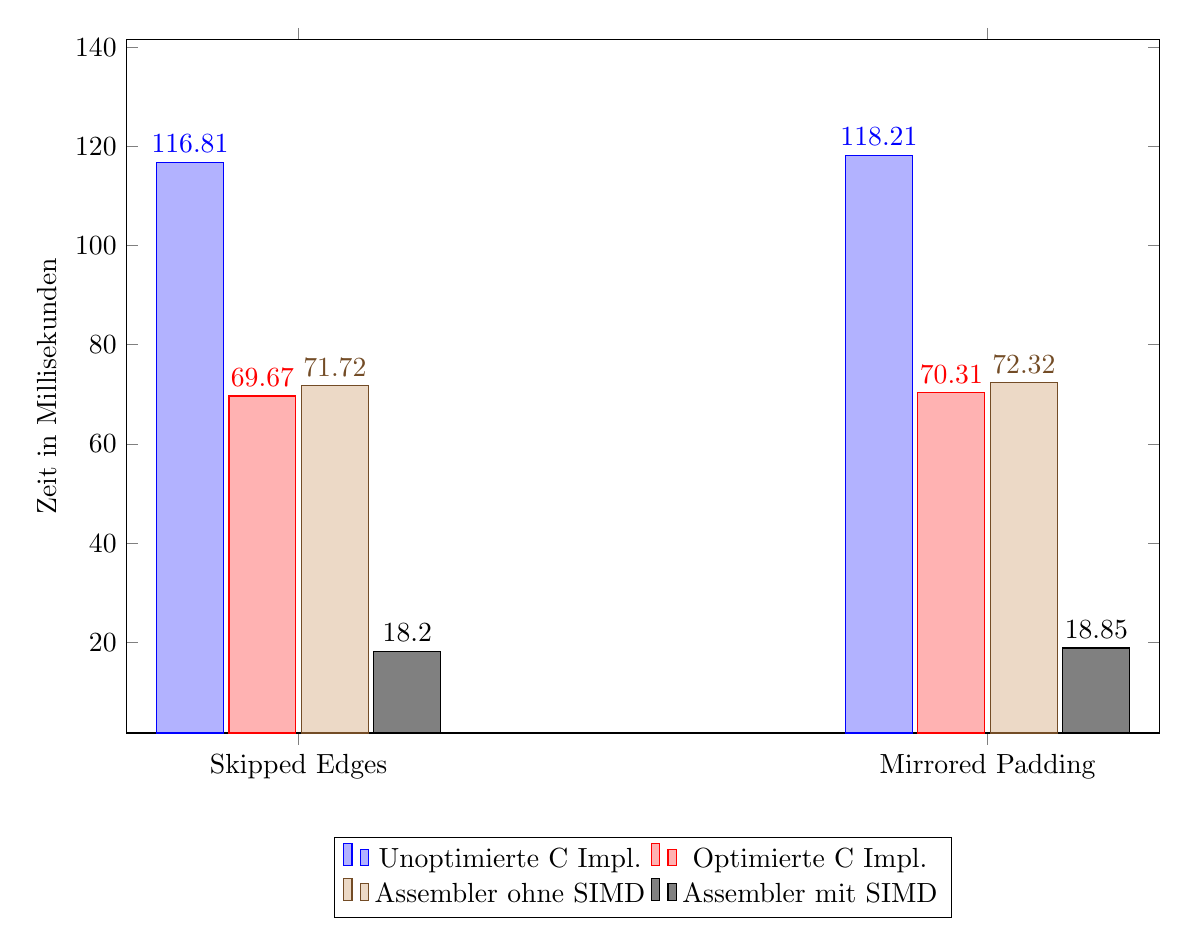
\begin{tikzpicture}
\begin{axis}[
	scale=1.25,
	ybar,
	ymin=25,
	x = 7cm,
	bar width = 0.85cm,
	symbolic x coords={Skipped Edges,Mirrored Padding},
	ylabel=Zeit in Millisekunden,
	enlargelimits=0.25,
	legend style={at={(0.5,-0.15)},anchor=north,legend columns=2},
	xtick=data,
    nodes near coords,
    nodes near coords align={vertical},
]
\addplot coordinates {(Skipped Edges,116.809100) (Mirrored Padding,118.211200)};
\addplot coordinates {(Skipped Edges,69.670600) (Mirrored Padding,70.309800)};
\addplot coordinates {(Skipped Edges,71.716800) (Mirrored Padding,72.324800)};
\addplot coordinates {(Skipped Edges,18.199600) (Mirrored Padding,18.854400)};
\legend{Unoptimierte C Impl.,Optimierte C Impl.,Assembler ohne SIMD,Assembler mit SIMD}
\end{axis}
\end{tikzpicture}
\end{center}
\end{figure}
\\Wie aus Abbildung \ref{Abb:1} ersichtlich wird, ist der Unterschied der durchschnittlichen Performanz beider Randstrategien marginal. Gravierend ist jedoch die jeweilige Differenz zwischen beiden Assembler-Implementierungen. Hier ist die SIMD-optimierte Version im Mittel mehr als dreifach so schnell, als die un-optimierte Implementierung. Durch die hohe Optimierungsstufe des Kompilierers ist die optimierte Version der C-Implementierung knapp, aber eindeutig schneller als die unoptimierte Assembler Version. Welchen Unterschied die Optimierungsstufe aber wirklich macht, wird durch Betrachten der nächsten Grafik deutlich. 

\begin{figure}[ht!]
\caption{Optimierungsstufe \textbf{\textit{O2}}}
\label{Abb:2}
\begin{center}
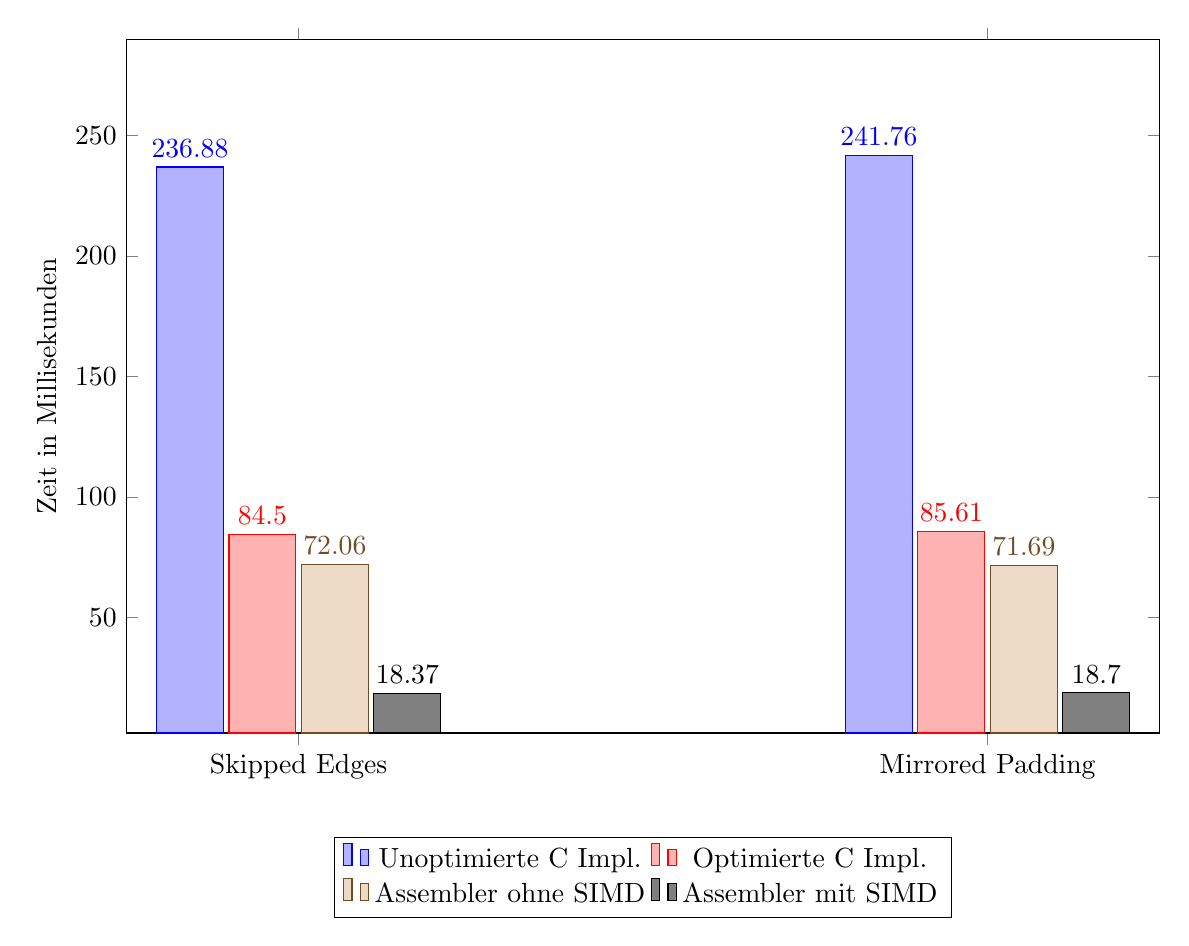
\begin{tikzpicture}
\begin{axis}[
	scale=1.25,
	ybar,
	ymin=50,
	x = 7cm,
	bar width = 0.85cm,
	symbolic x coords={Skipped Edges,Mirrored Padding},
	ylabel=Zeit in Millisekunden,
	enlargelimits=0.25,
	legend style={at={(0.5,-0.15)},anchor=north,legend columns=2},
	xtick=data,
    nodes near coords,
    nodes near coords align={vertical},
]
\addplot coordinates {(Skipped Edges,236.881300) (Mirrored Padding,241.756800)};
\addplot coordinates {(Skipped Edges,84.503900) (Mirrored Padding,85.612200)};
\addplot coordinates {(Skipped Edges,72.057200) (Mirrored Padding,71.692100)};
\addplot coordinates {(Skipped Edges,18.371300) (Mirrored Padding,18.702700)};
\legend{Unoptimierte C Impl.,Optimierte C Impl.,Assembler ohne SIMD,Assembler mit SIMD}
\end{axis}
\end{tikzpicture}
\end{center}
\end{figure}


In Abbildung \ref{Abb:2} ist eindeutig erkennbar, dass die unoptimierte C-Implementierung hier ein wenig mehr als das doppelte an Zeit, als bei der Kompilierung mit \textit{O3} braucht. 
In diesem Fall ist selbst die unoptimierte Assembler-Implementierung eindeutig schneller als die optimierte C-Version, da beide C-Implementierungen aufgrund mangelnder Optimierung Geschwindigkeit einbüßen müssen. Nahezu unverändert sind jedoch die Zeiten beider Assembler-Versionen. 
Ihre Funktionalität selbst wird durch den Kompilierer weder optimiert, noch verschlechtert.\\\\
Vergleicht man nun beide Grafiken miteinander, lässt sich eindeutig festellen, dass der einzige Unterschied das Rennen zwischen der optimierten C- und der unoptimierten Assembler - Implementierung ist. Während das \textit{O3} kompilierte C-Programm minimal schneller ist, so ist das \textit{O2} kompilierte C-Programm um eine ähnliche Differenz langsamer, als die jeweilige Assembler-Implementierung. Die unoptimierte C-Implementierung ist in jedem Szenario mit Abstand die langsamste, die optimierte Assembler-Implementierung die schnellste Version unseres Sobelfilters.
\section{Zusammenfassung und Ausblick}
% Effizienzvergleich 
% Ausblick: ?
In Kapitel \ref{Performanzanalyse} wird klar erkennbar, dass schon eine rudimentäre Implementierung gewisser Kernfunktionalitäten des Programms in Assembler implementiert annähernd so kurze Rechenzeit benötigt, wie eine optimierte Version des selben Algorithmus in C. Durch eine Optimierung des Assemblercodes mit Hilfe von SIMD-Operationen konnten wir sogar Laufzeiten erzielen, welche nur einen Bruchteil unserer bisherigen Zeiten darstellten.\\\\
Zusammenfassend lässt sich daher aus unseren gewonnenen Erkenntnissen schließen, dass es sich durchaus lohnen kann, gewisse Teile eines Algorithmus in C Programmen in optimierte Assembler-Implementierungen auszulagern, da hierdurch ein deutlicher Effizienzgewinn erzielt werden kann. Gerade bei kleineren Berechnungen/Operationen kann es sich jedoch auch lohnen, auf Inline-Assembler, auch integrierter Assemblercode genannt, zurückzugreifen. Auf diese Weise kann Assemblercode direkt in den Code höherer Programmiersprachen eingebettet und somit potenziell die Rechenzeit des Programms verkürzt werden.\\\\
\subsection{Mögliche Verbesserungen}
Eine Möglichkeit zur Laufzeitverbesserung unserer Assembler-Implementierungen bietet sich darin, die Berechnung der Quadrate (siehe Kapitel \ref{Quadratberechnung}) in 16 Bit Lanes, anstatt in 32 Bit Lanes durchzuführen. Durch die Vektorisierung fallen auf diese Weise weniger Produkte zu berechnen an, durch die potentiellen Overflows der Register ist jedoch mit einem Qualitätsverlust des Ergebnisses zu rechnen.\\\\
Eine weitere Möglichkeit zur marginalen Laufzeitverbesserung wäre, die vertikale Randbehandlung bei der \textit{Mirrored Padding}-Strategie direkt in den Kernalgorithmus in so weit zu integrieren, dass die linken und rechten Randpixel jeweils nicht doppelt geladen werden müssen und so load-Operationen eingespart werden könnten.
% TODO: Fuegen Sie Ihre Quellen der Datei Ausarbeitung.bib hinzu
% Referenzieren Sie diese dann mit \cite{}.
% Beispiel: CR2 ist ein Register der x86-Architektur~\cite{intel2017man}.
\newpage
\bibliographystyle{plain}
\bibliography{Ausarbeitung}{}

\end{document}
